\chapter{Extensiones al Programa Original}
\label{cap:extensiones}

Una vez comentadas las motivaciones, objetivos y planteamiento de trabajo, se tratarán los puntos en los que se ha trabajado para lograr la realización del proyecto. En este capítulo se incide en las extensiones y cambios realizados, tratados a bajo nivel y desde un punto de vista técnico.

\section{Adaptación para la ejecución de comandos desde la interfaz}

Como se ha comentado en varias ocasiones, siguiendo el objetivo principal de democratizar el uso de esta herramienta para perfiles no tecnológicos como psicólogos u otros profesionales, uno de los desafíos era hacer la aplicación disponible únicamente desde la interfaz, de modo que los usuarios interactúen con la interfaz para realizar todas las acciones.

Originalmente, si los usuarios querían elegir una simulación, ejecutarla o guardarla, por ejemplo, debían ejecutar estas acciones desde la terminal. Esto podría ser una barrera de entrada para ciertos usuarios que no estén familiarizados con estas tecnologías. El objetivo era hacerla accesible desde la interfaz únicamente.

Para conseguirlo, se plantearon ciertas opciones. Tras investigarlas, se tomó la decisión de optar por la opción representada en el diagrama de la figura \ref{fig:DiagramaComandos}, ya que no implicaría cambiar la arquitectura actual de la aplicación, en la cual son los comandos ejecutados en la terminal del backend los que indican las acciones a realizar y marcan las llamadas al modelo de lenguaje.

\begin{figure}[h]
	\centering
	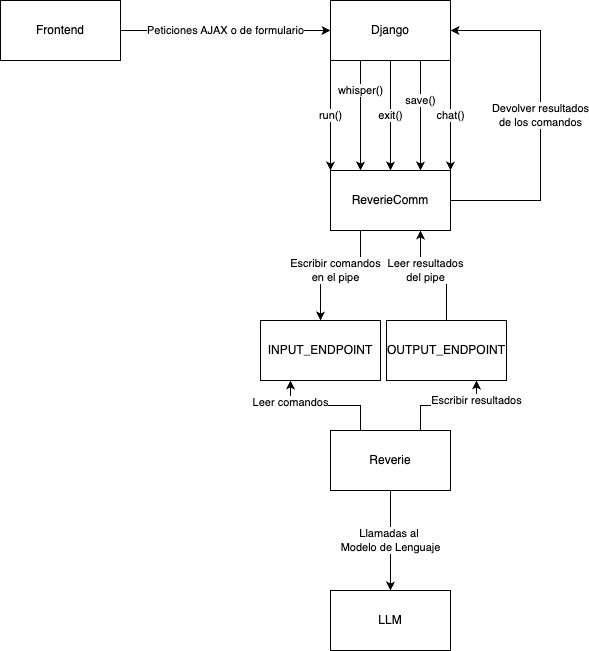
\includegraphics[width = 0.6\textwidth]{Imagenes/Vectorial/DiagramaComandos.png}
	\caption{Diagrama del estado de los comandos actualmente}
	\label{fig:DiagramaComandos}
\end{figure}

Como se aprecia en el diagrama, realmente siguen existiendo las llamadas de los comandos, pero se redirecciona para que se ejecuten desde la interacción con la interfaz. 

El flujo siempre comienza desde la propia interfaz, el front end. Mediante esta se hacen peticiones a django, que es el primero de los back ends, el que se encarga de cargar los datos, redirigir las vistas y comunicarse con el segundo de los backends (el que hemos llamado Reverie en el diagrama). Tras las llamadas a django, este se comunicará con una nueva clase, conocida como ReverieComm, para ejecutar los comandos mediante el uso de pipes. En una pipe habrá un fichero FIFO en el que se escribirán los comandos que deben de ser ejecutados, y el backend Reverie los leerá y ejecutará en orden, escribiendo la respuesta del modelo de lenguaje en otro fichero, para que sea leído por la clase ReverieComm y transmitido a Django, para que finalmente sea mostrado por pantalla mediante el front end.

De esta manera, logramos solucionar el problema de que los usuarios tengan que interactuar directamente con la terminal y al mismo tiempo no modificamos la arquitectura, ya que los comandos seguirán siendo ejecutados. 

\section{Interacción total con el sistema mediante la interfaz gráfica}

Uno de los retos para hacer el sistema fácilmente usable fue el cambiar la arquitectura y diseño de la aplicación para que todas las acciones se realizasen a través de la interfaz gráfica.

Consideramos esto algo central, ya que es uno de los pilares del presente trabajo, y algo que realmente aporta valor y ayuda a todos los perfiles como psicólogos, que sin saber cómo utilizar la aplicación, en unos minutos pueden estar experimentando con ella.

Es por ello, que a continuación, en las siguientes tablas, veremos la diferencia de cómo se hacían antes las acciones que ya estaban inicialmente implementadas, y cómo se hacen ahora con las modificaciones (en estas tablas solo se incluyen funcionalidades que ya estaban originalmente disponibles en el sistema original, no las nuevas implementadas en el presente trabajo):

\newcolumntype{L}{>{\raggedright\arraybackslash}X}

\begin{table}[H]
	\centering
	\begin{tabularx}{\linewidth}{|c|L|L|} 
		\hline
		\textbf{Funcionalidad} & \textbf{Antes} & \textbf{Después} \\ 
		\hline
		Crear simulación & En la terminal, insertar el nombre de una simulación base (con personajes predeterminados), elegir el nombre de la nueva simulación y crear la simulación & Desde la interfaz, ir a la pestaña de \textquotesingle Crear simulación\textquotesingle, rellenar las personalidades de los personajes deseados y clicar en \textquotesingle Empezar simulación\textquotesingle, automáticamente se redirije a la ejecución \\ 
		\hline
	\end{tabularx}
	\caption{Diferencias entre crear simulación antes y después}
	\label{table:tabla1}
\end{table}

Como se puede ver en la tabla \ref{table:tabla1}, inicialmente la tarea de crear una simulación era algo más complejo. Los usuarios debían acudir a la terminal, y ahí seleccionar una simulación base, la cual no permitía cambiar el número de personajes ni la personalidad de los mismos. Ahora, mediante la interfaz, se podrá seleccionar fácilmente el número de personajes y la personalidad, contexto y experiencias de cada uno.

\begin{table}[H]
	\centering
	\begin{tabularx}{\linewidth}{|c|L|L|} 
		\hline
		\textbf{Funcionalidad} & \textbf{Antes} & \textbf{Después} \\ 
		\hline
		Ejecutar simulación & Una vez creada una simulación, ir a la terminal y ejecutar el comando \textquotesingle run <número de steps>\textquotesingle, luego, ir a la interfaz y ver el resultado de la ejecución & En la pantalla de ejecución de simulación, darle al botón de run indicando el número de steps deseados, el resultado se verá en la interfaz directamente\\
		\hline
	\end{tabularx}
	\caption{Diferencias entre ejecutar simulación antes y después}
	\label{table:tabla2}
\end{table}

en la tabla \ref{table:tabla2} se aprecian las diferencias de cómo era antes ejecutar la simulación y cómo es ahora. Similar a como ocurría al crearla, lo que hemos hecho es evitar que los usuarios tengan que acudir a la terminal a ejecutar los pasos de la simulación, sino que se pueda hacer directamente desde el frontend.

\begin{table}[H]
	\centering
	\begin{tabularx}{\linewidth}{|c|L|L|} 
		\hline
		\textbf{Funcionalidad} & \textbf{Antes} & \textbf{Después} \\ 
		\hline
		Susurrar a un agente & Con la simulación corriendo, ejecutar en la terminal el comando \textquotesingle whisper <nombre del personaje> <mensaje>\textquotesingle & ir directamente al botón de susurro de cada personaje y añadir el mensaje deseado\\
		\hline
	\end{tabularx}
	\caption{Diferencias entre susurrar a un agente antes y después}
	\label{table:tabla3}
\end{table}

En la tercera de las tablas, la \ref{table:tabla3}, vemos cómo cambia la manera en la que susurramos a los agentes. Ahora es mucho más sencillo, desde la interfaz se buscará el agente con el que nos queremos comunicar y se enviará el mensaje a través de un modal. Antes, sin embargo, era necesario introducir también el nombre del personaje desde la interfaz.

\begin{table}[H]
	\centering
	\begin{tabularx}{\linewidth}{|c|L|L|} 
		\hline
		\textbf{Funcionalidad} & \textbf{Antes} & \textbf{Después} \\ 
		\hline
		Guardar simulación & En el modo ejecución de simulación, al considerarla terminada, ejecutar el comando \textquotesingle fin\textquotesingle & Al terminar, desde la página de ejecución de la simulación, tendremos la opción de guardar para ver la demo o guardar para continuar la simulación\\
		\hline
	\end{tabularx}
	\caption{Diferencias entre guardar simulación antes y después}
	\label{table:tabla4}
\end{table}

En cuanto a las diferencias a la hora de guardar una simulación, se pueden ver en la tabla \ref{table:tabla4}. A pesar de que antes era sencillo guardarlas, había que hacerlo desde la terminal también. Ahora, hemos eliminado eso, además de que se podrá elegir entre guardar para ver (redirige a la pestaña de visualizar) y guardar para continuar (que redirigirá a la pantalla de continuar simulación, para que se siga con la ejecución).

\begin{table}[H]
	\centering
	\begin{tabularx}{\linewidth}{|c|L|L|} 
		\hline
		\textbf{Funcionalidad} & \textbf{Antes} & \textbf{Después} \\ 
		\hline
		Salir sin guardar & En el modo ejecución, si ahora no se quiere guardar la simulación, el usuario debería ejecutar el comando \textquotesingle exit\textquotesingle & Al finalizar la simulación, si no se desea guardar, en la página de ejecución de simulación se clicará el botón de \textquotesingle Salir sin guardar\textquotesingle\\
		\hline
	\end{tabularx}
	\caption{Diferencias entre salir sin guardar simulación antes y después}
	\label{table:tabla5}
\end{table}

Similar a lo que ocurría con el caso de guardar, tenemos el caso de salir sin guardar, representado en la tabla \ref{table:tabla5}. En este caso, en lugar de guardar, simplemente salimos de la ejecución de la simulación, sin guardar la simulación y redirigiendo al usuario a la página de landing

\begin{table}[H]
	\centering
	\begin{tabularx}{\linewidth}{|c|L|L|} 
		\hline
		\textbf{Funcionalidad} & \textbf{Antes} & \textbf{Después} \\ 
		\hline
		Ver una demo & Ir al fichero \textquotesingle compress\_sim\_storage.py\textquotesingle y ejecutar la función compress, seleccionando la simulación deseada que se quiera comprimir. Una vez hecho esto, pegar en el navegador el nombre de la simulación comprimida, así como el step desde el que se quiere visualizar y la velocidad de reproducción, entonces, se mostrará por pantalla  & En la página de \textquotesingle Visualizar simulación\textquotesingle seleccionar la simulación que se desea ver, la velocidad de reproducción y el step desde el que se desea ver. Una vez seleccionado, se redirigirá automáticamente a la página de visualización\\
		\hline
	\end{tabularx}
	\caption{Diferencias entre ver una demo de simulación antes y después}
	\label{table:tabla6}
\end{table}

Finalmente, el caso de visualizar la demo de una simulación, reflejado en la tabla \ref{table:tabla6}. Antes era muy compleja la realización de esta acción. Los usuarios debían ejecutar una función para comprimir las simulaciones, encontrar las simulaciones en su propio dispositivo y pegar la dirección url directamente en el navegador. Esto resultaba muy complicado para el usuario. Ahora, simplemente guardando para visualizar en el futuro, los usuarios podrán acceder desde la página de \textquotesingle Visualizar simulación\textquotesingle a todas las simulaciones que tengan guardadas y así poder visualizarlas directamente, con un simple click, el resto de acciones son realizadas automáticamente.

\section{Funcionalidad de chat con los agentes en tiempo real}

Una de las funcionalidades novedosas, que no existían inicialmente en el sistema original, es la de chatear con los distintos agentes en tiempo real. Esto es, a medida que se va ejecutando la simulación, los usuarios podrán pausarla e interactuar con cada uno de los agentes mediante un chat. Se dice que este chat es en tiempo real ya que, dependiendo del momento en que el usuario pause la simulación, el agente mantendrá todos los recuerdos y se podrá interactuar con él, dando respuestas basadas en estos recuerdos y conocimientos.

Un caso de ejemplo de esta funcionalidad es si deseamos ver cómo un personaje va madurando y desarrollando una idea a lo largo de la simulación. Inicialmente, el usuario podría indicar al agente que tiene cierta creencia o pensamiento muy arraigado, y durante la simulación, forzar situaciones para que este agente se vea expuesto a otros puntos de vista que puedan modificar sus pensamientos.

A medida que el agente se ve expuesto a ciertas situaciones, puede ser que cambie parte de sus pensamientos y/o creencias. Por ello, es muy interesante esta funcionalidad de chat.

Si al principio de la simulación el usuario interactuase con el agente, este le diría el pensamiento que tan fuertemente había arraigado a su personalidad antes de comenzar la simulación. Sin embargo, a medida que avanza el tiempo, si se interactúa con el agente otras veces, puede que de respuestas diferentes y se vea cómo las ideas pueden ir cambiando y madurando.

La idea inicial de esta nueva funcionalidad era la de permitir a los usuarios como psicólogos puedan apreciar estos sutiles cambios en las mentalidades y traspasar este conocimiento a casos de humanos reales.

Además, otros casos reales de uso puede ser el estudio del resultado que tendría realizar ciertas acciones en algunas personas con cierta personalidad y ver cómo va avanzando el cambio en su personalidad, para saber qué conversaciones debemos tener con las personas para poder reestructurar su personalidad extrayendo los resultados de este experimento.

\section{Funcionalidad de resúmenes de las simulaciones}

Otra de las funcionalidades novedosas respecto al sistema inicial es la de generación de resúmenes automáticos al finalizar una simulación. Esta funcionalidad es otra de la que vimos con mayor sentido, ya que permitirá aportar un contexto a las simulaciones guardadas, para poder distinguirlas a simple vista.

Esta funcionalidad se pone en marcha automáticamente cuando el usuario guarda una simulación para visualizarla más tarde. Como se veía en la sección anterior, cuando se guarda una simulación para visualizar la demo, lo que se hace internamente es que la simulación se comprime mediante un script de python, el cual permite que se vean los personajes correctamente y se pueda gestionar la simulación para ser visualizada.

Una vez se comprime la simulación, se aprovecha y se realiza una llamada al modelo de lenguaje, pasando las memorias de todos los personajes con sus puntos de vista. Lo que hará el LLM con toda esta información es extrapolar todo lo que ha ido sucediendo durante la simulación, recogiendo así los momentos más interesantes y generando un resumen que será mostrado con el resto de la información en la vista de visualizar simulación.

El valor fundamental que aporta esta nueva simulación es que, si un usuario guarda varias simulaciones similares y se olvida de lo que había hecho, solamente viendo el nombre sería muy difícil distinguirlas. Sin embargo, con los resúmenes automáticos, podrá leer directamente esta síntesis y así distinguir rápidamente una simulación de la otra.

Estos resúmenes solamente se generan al guardar para simular por dos motivos: el primero es que se comprime la simulación y es más sencillo pasar esta nueva información al modelo de lenguaje, y la segunda es que si un usuario guarda una simulación para continuarla, significa que no la ha terminado completamente, sino que la quiere bifurcar a partir de ese punto, por lo que no se va a generar un resumen de una simulación que no está considerada como terminada.










